\documentclass[a4paper,12pt]{book}
\usepackage[utf8]{inputenc}
\title{}
\author{Rachel Morris}
\date{\today}

\usepackage{rachwidgets}
\usepackage{fancyhdr}
\usepackage{lastpage}
\usepackage{dirtree}
\usepackage{boxedminipage}

\setcounter{chapter}{3}
\setcounter{section}{0}
\newcommand{\laChapter}{3.1 Set Definitions and Operations\ }
\newcounter{question}

\newcommand{\laClass}{CS 210\ }
\newcommand{\laSemester}{Fall 2017\ }

\pagestyle{fancy}
\fancyhf{}
\lhead{\laClass \laSemester}
\chead{}
\rhead{Ch \laChapter}
\rfoot{\thepage\ of \pageref{LastPage}}
\lfoot{\scriptsize Compiled by Rachel Morris, last updated \today}

\renewcommand{\headrulewidth}{2pt}
\renewcommand{\footrulewidth}{1pt}

\begin{document}

    %\toggletrue{answerkey}
    \togglefalse{answerkey}

    %------------------------------------------------------------------%
    %- Exercise Begin -------------------------------------------------%
    %------------------------------------------------------------------%

    \section{Set Definitions and Operations}

    %------------------------------------------------------------------%
    \subsection{Common Sets}

        \begin{intro}{Common sets we will see in this chapter:}
            \begin{tabular}{l l}
                $\mathbb{N}$, the set of natural numbers &
                These numbers are ``counting
                \\ & numbers".
                This set contains 0 and
                \\ & positive integers.

                \\
                $\mathbb{Z}$, the set of integers &
                This set contains all integers:
                \\ & positive, negative, and zero.
                \\
                $\mathbb{Q}$, the set of rational numbers &
                This set contains all numbers that can
                \\ &  be characterized
                as ratios, such as $\frac{1}{2}$,
                \\ & $\frac{-17}{4}$,
                or even $\frac{3}{1}$.
                \\
                $\mathbb{R}$, the set of all real numbers &
                These can be thought of as decimal
                \\ & numbers with possibly
                unending
                \\ & strings of digits after
                the decimal point.
            \end{tabular}
        \end{intro}

        % - QUESTION --------------------------------------------------%
        \stepcounter{question}
        \begin{questionNOGRADE}{\thequestion}

            For the following numbers, which set(s) do they belong to?

            \begin{center}
                \begin{tabular}{| c | c | c | c | c |}
                    \hline
                    & $\mathbb{N}$ & $\mathbb{Z}$ & $\mathbb{Q}$ & $\mathbb{R}$
                    \\ \hline
                    10 & & & &
                    \\ \hline
                    -5 & & & &
                    \\ \hline
                    $12/6$ & & & &
                    \\ \hline
                    $\pi$ & & & &
                    \\ \hline
                    2.40 & & & &
                    \\ \hline
                \end{tabular}
            \end{center}

        \end{questionNOGRADE}


        % - QUESTION --------------------------------------------------%
        \stepcounter{question}
        \begin{questionNOGRADE}{\thequestion}
            Give examples for each of the following types of sets:

            \begin{enumerate}
                \item[a.]   List three numbers that are in the
                    set of all integers, $\mathbb{Z}$,
                    but are NOT in the set of natural numbers,
                    $\mathbb{N}$.
                    \solution{}{ ~\\ }

                \item[b.]   List three numbers that are in the
                    set of rational numbers, $\mathbb{Q}$,
                    but are NOT in the set of integers,
                    $\mathbb{Z}$.
                    \solution{}{ ~\\ }

                \item[c.]   List three numbers that are in the
                    set of all real numbers $\mathbb{R}$,
                    but are NOT in the set of rational numbers,
                    $\mathbb{Q}$.
                    \solution{}{ ~\\ }
            \end{enumerate}
        \end{questionNOGRADE}

        \newpage

        \begin{intro}{Writing out sets}
            When we are building a discrete (finite) set,
            we usually give the set a capital letter as its
            identifier. Then, the elements of the set are written
            within curly-braces, like this:

            $$ A = \{ 2, 4, 6, 8 \} $$

            The elements here are 2, 4, 6, and 8.
            The index of the element 2 is 1 - it is
            at position 1 of the set - so $A_1 = 2$.
        \end{intro}


        % - QUESTION --------------------------------------------------%
        \stepcounter{question}
        \begin{questionNOGRADE}{\thequestion}

            Create sets that meet the following criteria.
            Give the sets any letter identifier that you want.

            \begin{enumerate}
                \item[a.]   All elements of the set are odd integers.
                    \solution{}{ ~\\~\\ }

                \item[b.]   All elements of the set are fractions
                    such that, when divided, they result in
                    an infinite string of numbers to the right
                    of the decimal place (e.g., $3.333333\bar{3}$...)
                    \solution{}{ ~\\~\\ }

                \item[c.]   Create two sets of integers, where
                    the two sets have exactly two elements in common.
                    \solution{}{ ~\\~\\ }

                \item[d.]   Create two sets of natural numbers,
                    where the two sets have NO elements in common.
                    \solution{}{ ~\\~\\ }

                \item[e.]   Create a set that is empty.
                    \solution{}{ ~\\~\\ }
            \end{enumerate}

        \end{questionNOGRADE}

        \newpage

        \subsection{Subsets}

        \begin{intro}{Subsets and existence within sets:}
            ~\\
            \begin{tabular}{l l}
                $x$ exists in $A$ &
                    The notation $x \in A$ means ``$x$ is an element of $A$"
                    \\ &
                    which means that $x$ is one of the member elements
                    \\ & of $A$.
                \\ \\
                $A$ is a subset of $B$ &
                    $A$ is a subset of $B$ (written as $A \subseteq B$) if
                    \\ &
                    every element in $A$ is also an element in $B$.
                    \\ &
                    Formally, this means that for every $x$, if $x \in A$,
                    \\ & then $x \in B$.
                \\ \\
                $A$ is equal to $B$ &
                    $A$ is equal to $B$ (written $A = B$) means that
                    \\ &
                    $A$ and $B$ have exactly the same members. This is
                    \\ &
                    expressed formally by saying, $A \subseteq B$ and $B \subseteq A$.
                \\ \\
                An Empty set &
                    A set that contains no elements is called an empty
                    \\ & set,
                    and it is denoted by $\{ \}$ or $\emptyset$.
                \\ \\
                The Universal set &
                    For any given discussion, all the sets will be subsets
                    \\ & of a larger set called the universal set (or universe)
                    \\ &We commonly use the letter $U$ to denote this set.
            \end{tabular}
        \end{intro}


        % - QUESTION --------------------------------------------------%
        \stepcounter{question}
        \begin{questionNOGRADE}{\thequestion}

            Given theset sets:

            \begin{tabular}{l l l}
                $U = \{-2, -1, 1, 2, 3, 4, 5, 6\}$ &
                $A = \{1, 1, 2, 2, 2, 4, 4\}$ &
                $B = \{-2, 2\}$ \\
                $C = \{1, 2, 4, 5, 6\}$ &
                $D = \{6, 5, 4, 2, 1\}$ &
                $E = \{1, 4\}$
            \end{tabular}

            \begin{enumerate}
                \item[a.] Which of these statements are true? Mark with a $\checkmark$

                \begin{tabular}{l l l}
                    a. $B \subseteq A$      \solution{ \xmark }{ \fitb } &
                    b. $B \subseteq E$      \solution{ \xmark }{ \fitb } &
                    c. $E \subseteq A$      \solution{ \checkmark }{ \fitb }
                    \\
                    d. $A \subseteq U$      \solution{ \checkmark }{ \fitb } &
                    e. $D \subseteq C$      \solution{ \checkmark }{ \fitb } &
                    f. $C \subseteq D$      \solution{ \checkmark }{ \fitb }
                    \\
                    g. $B \subseteq \mathbb{N}$ \solution{ \xmark }{ \fitb } &
                    h. $E \subseteq \mathbb{Z}$ \solution{ \checkmark }{ \fitb } &
                    i. $A \subseteq C$      \solution{ \checkmark }{ \fitb }
                \end{tabular}

                \item[b.] Fill in the blanks with either
                    $\subseteq$ (is a subset of), or
                    $\not\subseteq$ (is not a subset of), or
                    $=$ (is equal to) for the following:

                \begin{tabular}{l l l}
                    a. $C$ \solution{ = }{\fitb} $D$ &
                    b. $B$ \solution{ $\subseteq$ }{\fitb} $U$ &
                    c. $A$ \solution{ $\not\subseteq$}{\fitb} $E$
                \end{tabular}
            \end{enumerate}

        \end{questionNOGRADE}

        \newpage

        \subsection{Intersections, unions, and differences}

        \begin{intro}{\ }
            \begin{tabular}{l l}
                Intersection of $A$ and $B$, $A \cap B$ &
                    Is the set that contains those \\ &
                    elements common to both $A$ and $B$. \\ &
                    In set-builder notation, we write: \\ &
                    $A \cap B = \{ x \in U : x \in A \land x \in B \}$
                    \\
                \\
                Union of $A$ and $B$, $A \cup B$ &
                    Is the set that contains those \\ &
                    elements in either set $A$ or $B$. \\ &
                    In set-builder notation, we write: \\ &
                    $A \cup B = \{ x \in U: x \in A \lor x \in B \}$
                    \\
                \\
                Difference of $A$ and $B$, $A - B$ &
                    Is the set that contains those elements \\ &
                    in $A$ which are NOT in $B$. In set- \\&
                    buidler notation, we write: \\ &
                    $A - B = \{ x \in U : x \in A \land x \not\in B \}$
                    \\
                \\
                Disjoint sets &
                    Sets $A$ and $B$ are disjoint if \\ &
                    $A \cap B = \emptyset$.
                \\ \\
                Complement of $A$, $A'$ &
                    Given a set $A$ with elements from the \\ &
                    universe $U$, the complement of $A$ \\ &
                    (written $A'$) is the set that contains \\ &
                    those elemnets of the universal set $U$ \\ &
                    which are not in $A$. That is, \\ &
                    $A' = U-A$.
                    \\
            \end{tabular}

            ~\\
            Venn diagrams are used to visually represent relationships
            between sets. Set $A$ and set $B$ (or more) are drawn
            as overalpping circles, and the shaded-in region is the
            resulting set based on the \textit{intersection},
            \textit{union}, \textit{complement}, or \textit{difference}
            operations.

            \begin{center}
                \begin{tabular}{c c c c}
                    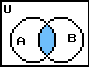
\includegraphics[width=2.5cm]{images/3-1-intersection.png}
                    &
                    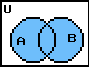
\includegraphics[width=2.5cm]{images/3-1-union.png}
                    &
                    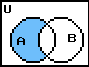
\includegraphics[width=2.5cm]{images/3-1-difference.png}
                    &
                    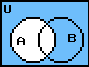
\includegraphics[width=2.5cm]{images/3-1-complement.png}
                    \\
                    $A \cap B$ &
                    $A \cup B$ &
                    $A - B$ &
                    $A'$
                \end{tabular}
            \end{center}

        \end{intro}

        \newpage

        % - QUESTION --------------------------------------------------%
        \stepcounter{question}
        \begin{questionNOGRADE}{\thequestion}

            For the following set operations, color in the Venn diagrams.

            \begin{center}
                \begin{tabular}{c c c}
                    $A \cap B$ &
                    $A \cap C$ &
                    $(A \cap B) \cup C$
                    \\
                    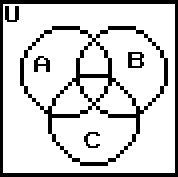
\includegraphics[width=4cm]{images/venndiagram.png} &
                    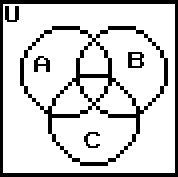
\includegraphics[width=4cm]{images/venndiagram.png} &
                    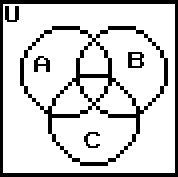
\includegraphics[width=4cm]{images/venndiagram.png}
                    \\
                    $B \cup C$ &
                    $A \cap (B \cup C)$ &
                    $B - C$
                    \\
                    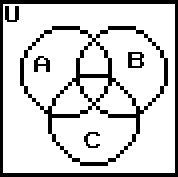
\includegraphics[width=4cm]{images/venndiagram.png} &
                    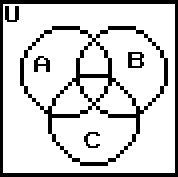
\includegraphics[width=4cm]{images/venndiagram.png} &
                    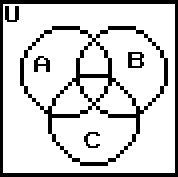
\includegraphics[width=4cm]{images/venndiagram.png}
                    \\
                    $A'$ &
                    $(A \cup B) - B$ &
                    $A \cup (B - C)$
                    \\
                    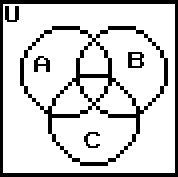
\includegraphics[width=4cm]{images/venndiagram.png} &
                    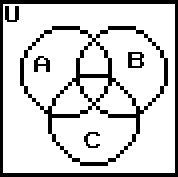
\includegraphics[width=4cm]{images/venndiagram.png} &
                    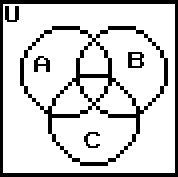
\includegraphics[width=4cm]{images/venndiagram.png}
                    \\
                    $(A \cap B) \cup (A \cap C)$ &
                    $(A \cup B) \cap (A \cup C)$ &
                    $(A \cup B \cup C)$
                    \\
                    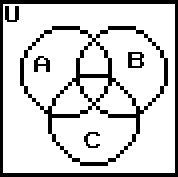
\includegraphics[width=4cm]{images/venndiagram.png} &
                    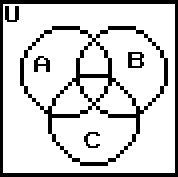
\includegraphics[width=4cm]{images/venndiagram.png} &
                    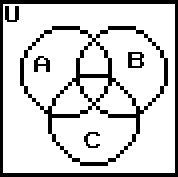
\includegraphics[width=4cm]{images/venndiagram.png}
                \end{tabular}
            \end{center}

        \end{questionNOGRADE}

        \newpage

        % - QUESTION --------------------------------------------------%
        \stepcounter{question}
        \begin{questionNOGRADE}{\thequestion}

            Given the following sets, compute the set operations and prove
            the following statements.

            \begin{tabular}{l l l l}
                $U = \{1, 2, 3, 4, 5, 6, 7, 8 \} $ &
                $A = \{1, 3, 5\}$ &
                $B = \{1, 2, 3, 4\}$ &
                $C = \{1, 2, 5, 6, 8\}$
            \end{tabular}

            \begin{enumerate}
                \item[a.]   $A \cap (B \cup C) = (A \cap B) \cup (A \cap C)$
                    \solution{}{ ~\\ \raisebox{0pt}[4cm][0pt]{  } }

                \item[b.]   $(A \cup B)' = A' \cap B'$
                    \solution{}{ ~\\ \raisebox{0pt}[4cm][0pt]{  } }

                \item[c.]   $A \cap (A \cup B) = A$
                    \solution{}{ ~\\ \raisebox{0pt}[4cm][0pt]{  } }
            \end{enumerate}

        \end{questionNOGRADE}

        \newpage

        \subsection{Set-builder notation}

        \begin{intro}{\ }
            It is impractical to try to list every element of a set.
            We use set-builder notation to describe most sets.
            There are two different forms of set-builder notation:

            ~\\
            A \textbf{Property Description} is of the form,
            ``The set of all $x$ in $u$, such that $x$ is \fitb."
            The blank is some \textit{property} of $x$, which
            determines whether an element of $U$ is or is not in the set.

            \begin{itemize}
                \item   The set of even integers:
                    $\{ x \in \mathbb{Z} : x = 2y$ for some $y \in \mathbb{Z} \}$
                \item   The set of real numbers bigger than 10:
                    $\{ x \in \mathbb{R} : x > 10 \}$
            \end{itemize}

            ~\\
            A \textbf{Form Description} is of the form,
            ``All numbers of the form \fitb, where $x$ is in the set $D$."
            The first part will be some equation (like ``$2x$" for even).
            
            \begin{itemize}
                \item   The set of even integers:
                    $\{ 2k : k \in \mathbb{Z} \}$
                \item   The set of perfect square integers:
                    $\{ m^{2} : m \in \mathbb{Z} \}$
            \end{itemize}
        \end{intro}

        % - QUESTION --------------------------------------------------%
        \stepcounter{question}
        \begin{questionNOGRADE}{\thequestion}

            Write the following in 
            \textbf{property description} set-builder notation, using
            the steps given to help you figure it out.

            \begin{center}
                ``The set of all odd integers"
            \end{center}

            \begin{itemize}
                \item[Step 1.]  Using $x$ as the variable, what set does $x$ belong in? \tab
                    $x \in $ \solution{ $\mathbb{Z}$ }{ \fitb }

                \item[Step 2.]  In English, how would you describe $x$?
                    \tab[1.2cm] $x$ is \solution{ an odd integer }{ \fitb[3cm] }

                \item[Step 3.]  How would you write Step 2 symbolically? \tab[1.5cm]
                    $x = $ \solution{ $2k + 1$ }{ \fitb[2cm]}

                \item[Step 4.]  For the \textbf{Property Description}, \\
                    it should be in the form \textit{ ( \{ set : property \} ) }. Fill out the following:

                    \begin{tabular}{ c c c c c c c c c}
                        $\{ x \in$
                        & \solution{$\mathbb{Z}$}{\fitb} & :
                        & \solution{$x = 2k+1$}{\fitb[2cm]} & for some
                        & \solution{$k$}{\fitb} & $\in$
                        & \solution{\mathbb{Z}}{\fitb} & $\}$ \\
                        & Step 1 set & & Step 3 & & $2^{nd}$ var & & Step 1 set
                    \end{tabular}

                    ~\\
                    \footnotesize (The 2nd variable is part of the equation in Step 3.)
            \end{itemize}

        \end{questionNOGRADE}

        \newpage

    
        % - QUESTION --------------------------------------------------%
        \stepcounter{question}
        \begin{questionNOGRADE}{\thequestion}

            Write the following in 
            \textbf{form description} set-builder notation, using
            the steps given to help you figure it out.

            \begin{center}
                ``The set of all integers divisible by 3"
            \end{center}

            \begin{itemize}
                \item[Step 1.]  Using $x$ as the variable, what set does $x$ belong in? \tab
                    $x \in $ \solution{ $\mathbb{Z}$ }{ \fitb }

                \item[Step 2.]  In English, how would you describe $x$?
                    \tab[1.2cm] $x$ is \solution{ an odd integer }{ \fitb[3cm] }

                \item[Step 3.]  How would you write Step 2 symbolically? \tab[1.5cm]
                    $x = $ \solution{ $2k + 1$ }{ \fitb[2cm]}

                \item[Step 4.]  For the \textbf{Form Description}, \\
                    it should be in the form \textit{ ( \{ form : set \} ) }. Fill out the following:

                    \begin{tabular}{ c c c c c c c c}
                        $\{$
                        & \solution{$3m$}{\fitb[2cm]} & :
                        & \solution{$m$}{\fitb} & $\in$
                        & \solution{$\mathbb{Z}$}{\fitb} & $\}$ \\
                        & Step 3 RHS & &
                        Step 3 RHS variable & &
                        Step 1 set
                    \end{tabular}

                    ~\\
                    \footnotesize (Here, you don't use the full equation from Step 3; you remove the $x$.)
            \end{itemize}

        \end{questionNOGRADE}



\end{document}








